\section{Base Software Development} \label{sec:software}

Neural networks and feature descriptors are decided to be used for cat and dog classification. Since embedded electronic computers are not capable of doing mass works, it is concluded that a server is going to be used. As a result, it became a must to transfer data from the embedded system to the powerful computer. The transfer process is done over network socket with TCP protocol.

To transfer data properly and make the whole system consistent, a schema of software overview is designed. Figure \ref{fig:overallView} shows the rough schema that how the network is constructed and related to the other components of the project such as computer vision, database, starting cat feeder.

\begin{figure}[htp]
    \centering
    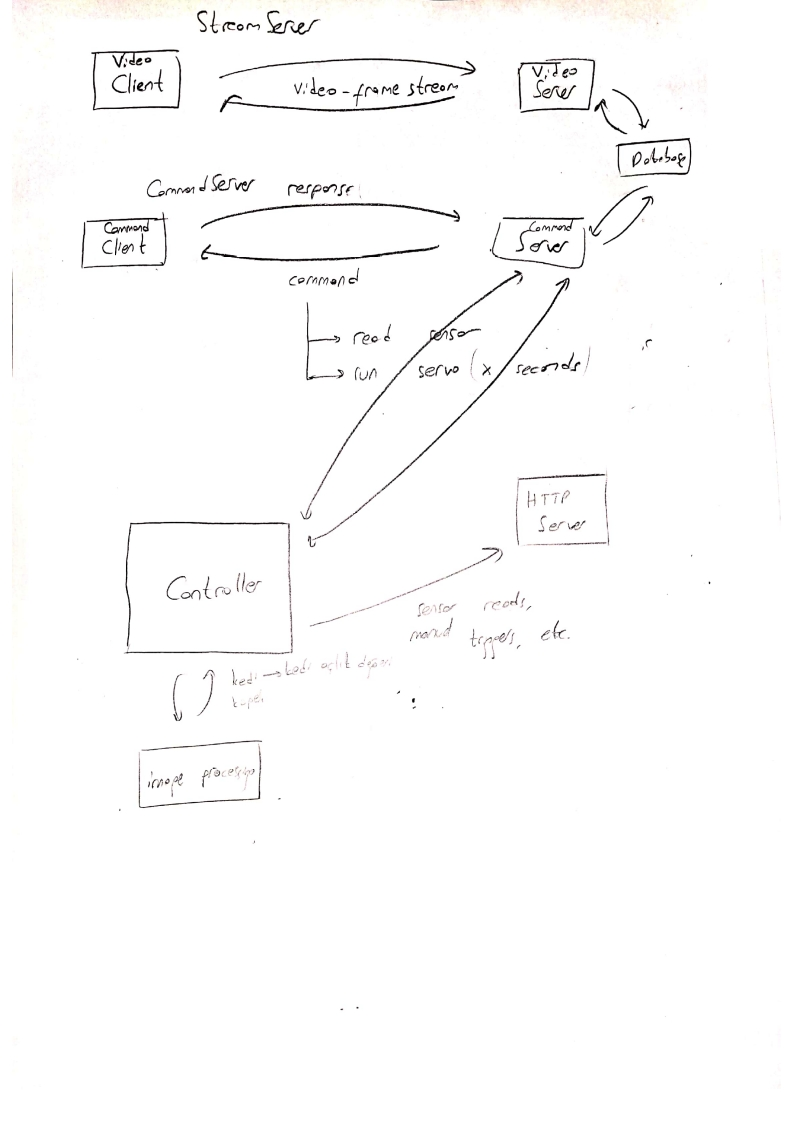
\includegraphics[width=0.98\linewidth]{SchemaSharpened.jpg}
    \caption{Overall System Schema}
    \label{fig:overallView}
\end{figure}

Native implementation of python of ServerSocket and Socket objects are used. This part of the work includes the data transfer, video streaming and frame transfer, command transfer and response. This week is mainly about transferring a single frame over network and abstract object structures for client-server and camera driver objects. More specifically, camera driver(CameraDriver.py) and server-client(ServerClient.py) source files are started and some basic functionalities are added. Note that currenly the source code is being developed under pi branch in GitHub which will then be rebased so that minimum congestion arises.

Parameter optimization for the data transfer is the another factor which affect the data transfer performance and stability of the transferred image. Using greater number of frames and low data buffer sizes, the image is transferred partially, or even the first segments are broken which caused the corrupted data. The system is still needed to be improved and integrated with the computer vision work group of the project.